
\documentclass[letterpaper,hide notes,xcolor={table,svgnames},pdftex,10pt]{beamer}
\def\showexamples{t}


%\usepackage[svgnames]{xcolor}

%% Demo talk
%\documentclass[letterpaper,notes=show]{beamer}

\usecolortheme{crane}
\setbeamertemplate{navigation symbols}{}

\usetheme{MyPittsburgh}
%\usetheme{Frankfurt}

%\usepackage{tipa}

\usepackage{hyperref}
\usepackage{graphicx,xspace}
\usepackage[normalem]{ulem}
\usepackage{multicol}
\usepackage{amsmath,amssymb,amsthm,graphicx,xspace}
\newcommand\SF[1]{$\bigstar$\footnote{SF: #1}}

\usepackage[default]{sourcesanspro}
\usepackage[T1]{fontenc}
\usepackage[scaled]{beramono}
\usepackage{tikzpagenodes}

\newcounter{tmpnumSlide}
\newcounter{tmpnumNote}


% old question code
%\newcommand\question[1]{{$\bigstar$ \small \onlySlide{2}{#1}}}
% \newcommand\nquestion[1]{\ifdefined \presentationonly \textcircled{?} \fi \note{\par{\Large \textbf{?}} #1}}
% \newcommand\nanswer[1]{\note{\par{\Large \textbf{A}} #1}}


 \newcommand\mnote[1]{%
   \addtocounter{tmpnumSlide}{1}
   \ifdefined\showcues {~\tiny\fbox{\arabic{tmpnumSlide}}}\fi
   \note{\setlength{\parskip}{1ex}\addtocounter{tmpnumNote}{1}\textbf{\Large \arabic{tmpnumNote}:} {#1\par}}}

\newcommand\mmnote[1]{\note{\setlength{\parskip}{1ex}#1\par}}

%\newcommand\mnote[2][]{\ifdefined\handoutwithnotes {~\tiny\fbox{#1}}\fi
% \note{\setlength{\parskip}{1ex}\textbf{\Large #1:} #2\par}}

%\newcommand\mnote[2][]{{\tiny\fbox{#1}} \note{\setlength{\parskip}{1ex}\textbf{\Large #1:} #2\par}}

\newcommand\mquestion[2]{{~\color{red}\fbox{?}}\note{\setlength{\parskip}{1ex}\par{\Large \textbf{?}} #1} \note{\setlength{\parskip}{1ex}\par{\Large \textbf{A}} #2\par}\ifdefined \presentationonly \pause \fi}

\newcommand\blackboard[1]{%
\ifdefined   \showblackboard
  {#1}
  \else {\begin{center} \fbox{\colorbox{blue!30}{%
         \begin{minipage}{.95\linewidth}%
           \hspace{\stretch{1}} Some space intentionally left blank; done at the blackboard.%
         \end{minipage}}}\end{center}}%
         \fi%
}



%\newcommand\q{\tikz \node[thick,color=black,shape=circle]{?};}
%\newcommand\q{\ifdefined \presentationonly \textcircled{?} \fi}

\usepackage{listings}
\lstset{basicstyle=\footnotesize\ttfamily,
	breaklines=true,
	aboveskip=15pt,
  	belowskip=15pt,
	frame=lines,
	numbers=left, basicstyle=\scriptsize, numberstyle=\tiny, stepnumber=0, numbersep=2pt
}

\usepackage{siunitx}
\newcommand\sius[1]{\num[group-separator = {,}]{#1}\si{\micro\second}}
\newcommand\sims[1]{\num[group-separator = {,}]{#1}\si{\milli\second}}
\newcommand\sins[1]{\num[group-separator = {,}]{#1}\si{\nano\second}}
\sisetup{group-separator = {,}, group-digits = true}

%% -------------------- tikz --------------------
\usepackage{tikz}
\usetikzlibrary{positioning}
\usetikzlibrary{arrows,backgrounds,automata,decorations.shapes,decorations.pathmorphing,decorations.markings,decorations.text,decorations.pathreplacing}

\tikzstyle{place}=[circle,draw=blue!50,fill=blue!20,thick, inner sep=0pt,minimum size=6mm]
\tikzstyle{transition}=[rectangle,draw=black!50,fill=black!20,thick, inner sep=0pt,minimum size=4mm]

\tikzstyle{block}=[rectangle,draw=black, thick, inner sep=5pt]
\tikzstyle{bullet}=[circle,draw=black, fill=black, thin, inner sep=2pt]

\tikzstyle{pre}=[<-,shorten <=1pt,>=stealth',semithick]
\tikzstyle{post}=[->,shorten >=1pt,>=stealth',semithick]
\tikzstyle{bi}=[<->,shorten >=1pt,shorten <=1pt, >=stealth',semithick]

\tikzstyle{mut}=[-,>=stealth',semithick]

\tikzstyle{treereset}=[dashed,->, shorten >=1pt,>=stealth',thin]

\usepackage{ifmtarg}
\usepackage{xifthen}
\makeatletter
% new counter to now which frame it is within the sequence
\newcounter{multiframecounter}
% initialize buffer for previously used frame title
\gdef\lastframetitle{\textit{undefined}}
% new environment for a multi-frame
\newenvironment{multiframe}[1][]{%
\ifthenelse{\isempty{#1}}{%
% if no frame title was set via optional parameter,
% only increase sequence counter by 1
\addtocounter{multiframecounter}{1}%
}{%
% new frame title has been provided, thus
% reset sequence counter to 1 and buffer frame title for later use
\setcounter{multiframecounter}{1}%
\gdef\lastframetitle{#1}%
}%
% start conventional frame environment and
% automatically set frame title followed by sequence counter
\begin{frame}%
\frametitle{\lastframetitle~{\normalfont(\arabic{multiframecounter})}}%
}{%
\end{frame}%
}
\makeatother

\makeatletter
\newdimen\tu@tmpa%
\newdimen\ydiffl%
\newdimen\xdiffl%
\newcommand\ydiff[2]{%
    \coordinate (tmpnamea) at (#1);%
    \coordinate (tmpnameb) at (#2);%
    \pgfextracty{\tu@tmpa}{\pgfpointanchor{tmpnamea}{center}}%
    \pgfextracty{\ydiffl}{\pgfpointanchor{tmpnameb}{center}}%
    \advance\ydiffl by -\tu@tmpa%
}
\newcommand\xdiff[2]{%
    \coordinate (tmpnamea) at (#1);%
    \coordinate (tmpnameb) at (#2);%
    \pgfextractx{\tu@tmpa}{\pgfpointanchor{tmpnamea}{center}}%
    \pgfextractx{\xdiffl}{\pgfpointanchor{tmpnameb}{center}}%
    \advance\xdiffl by -\tu@tmpa%
}
\makeatother
\newcommand{\copyrightbox}[3][r]{%
\begin{tikzpicture}%
\node[inner sep=0pt,minimum size=2em](ciimage){#2};
\usefont{OT1}{phv}{n}{n}\fontsize{4}{4}\selectfont
\ydiff{ciimage.south}{ciimage.north}
\xdiff{ciimage.west}{ciimage.east}
\ifthenelse{\equal{#1}{r}}{%
\node[inner sep=0pt,right=1ex of ciimage.south east,anchor=north west,rotate=90]%
{\raggedleft\color{black!50}\parbox{\the\ydiffl}{\raggedright{}#3}};%
}{%
\ifthenelse{\equal{#1}{l}}{%
\node[inner sep=0pt,right=1ex of ciimage.south west,anchor=south west,rotate=90]%
{\raggedleft\color{black!50}\parbox{\the\ydiffl}{\raggedright{}#3}};%
}{%
\node[inner sep=0pt,below=1ex of ciimage.south west,anchor=north west]%
{\raggedleft\color{black!50}\parbox{\the\xdiffl}{\raggedright{}#3}};%
}
}
\end{tikzpicture}
}


%% --------------------

%\usepackage[excludeor]{everyhook}
%\PushPreHook{par}{\setbox0=\lastbox\llap{MUH}}\box0}

%\vspace*{\stretch{1}

%\setbox0=\lastbox \llap{\textbullet\enskip}\box0}

\setlength{\parskip}{\fill}

\newcommand\noskips{\setlength{\parskip}{1ex}}
\newcommand\doskips{\setlength{\parskip}{\fill}}

\newcommand\xx{\par\vspace*{\stretch{1}}\par}
\newcommand\xxs{\par\vspace*{2ex}\par}
\newcommand\tuple[1]{\langle #1 \rangle}
\newcommand\code[1]{{\sf \footnotesize #1}}
\newcommand\ex[1]{\uline{Example:} \ifdefined \presentationonly \pause \fi
  \ifdefined\showexamples#1\xspace\else{\uline{\hspace*{2cm}}}\fi}

\newcommand\ceil[1]{\lceil #1 \rceil}


\AtBeginSection[]
{
   \begin{frame}
       \frametitle{Outline}
       \tableofcontents[currentsection]
   \end{frame}
}



\pgfdeclarelayer{edgelayer}
\pgfdeclarelayer{nodelayer}
\pgfsetlayers{edgelayer,nodelayer,main}

\tikzstyle{none}=[inner sep=0pt]
\tikzstyle{rn}=[circle,fill=Red,draw=Black,line width=0.8 pt]
\tikzstyle{gn}=[circle,fill=Lime,draw=Black,line width=0.8 pt]
\tikzstyle{yn}=[circle,fill=Yellow,draw=Black,line width=0.8 pt]
\tikzstyle{empty}=[circle,fill=White,draw=Black]
\tikzstyle{bw} = [rectangle, draw, fill=blue!20, 
    text width=4em, text centered, rounded corners, minimum height=2em]
    
    \newcommand{\CcNote}[1]{% longname
	This work is licensed under the \textit{Creative Commons #1 3.0 License}.%
}
\newcommand{\CcImageBy}[1]{%
	\includegraphics[scale=#1]{creative_commons/cc_by_30.pdf}%
}
\newcommand{\CcImageSa}[1]{%
	\includegraphics[scale=#1]{creative_commons/cc_sa_30.pdf}%
}
\newcommand{\CcImageNc}[1]{%
	\includegraphics[scale=#1]{creative_commons/cc_nc_30.pdf}%
}
\newcommand{\CcGroupBySa}[2]{% zoom, gap
	\CcImageBy{#1}\hspace*{#2}\CcImageNc{#1}\hspace*{#2}\CcImageSa{#1}%
}
\newcommand{\CcLongnameByNcSa}{Attribution-NonCommercial-ShareAlike}

\newenvironment{changemargin}[1]{% 
  \begin{list}{}{% 
    \setlength{\topsep}{0pt}% 
    \setlength{\leftmargin}{#1}% 
    \setlength{\rightmargin}{1em}
    \setlength{\listparindent}{\parindent}% 
    \setlength{\itemindent}{\parindent}% 
    \setlength{\parsep}{\parskip}% 
  }% 
  \item[]}{\end{list}} 




\title{Lecture 17 --- C/C++11 Memory Model }

\author{Patrick Lam \& Jeff Zarnett \\ \small \texttt{p.lam@ece.uwaterloo.ca}, \texttt{jzarnett@uwaterloo.ca}}
\institute{Department of Electrical and Computer Engineering \\
  University of Waterloo}
\date{\today}


\begin{document}

\begin{frame}
  \titlepage

 \end{frame}

%%%%%%%%%%%%%%%%%%%%%%%%%%%%%%%%%%%%%%%%%%%%%%%%%%%%%%%%%%%%%%%%%%%%%%%%%%%%%%%%
\begin{frame}[fragile]
  \frametitle{Language Support: Before C/C++11}

%http://www.quora.com/C++-programming-language/How-are-the-threading-and-memory-models-different-in-C++-as-compared-to-C

  
    Before C/C++11: \\ \qquad no language-level definition of threads.\\[1em]

    Not even a well-formed question to ask what this means:\\[.5em]
    \begin{tabular}{ll}
      \begin{minipage}{.2\textwidth}
        Thread 1:
        \begin{lstlisting}
  foo = 7;
  bar = 42;
        \end{lstlisting}
      \end{minipage} &
      \begin{minipage}{.4\textwidth}
        Thread 2:
        \begin{lstlisting}
  printf("%d\n", foo);
  printf("%d\n", bar);
        \end{lstlisting}
      \end{minipage}
    \end{tabular}
    ~\\[1em]
    \only<2>{pre C/C++11: no such thing as a thread!}
    
  
\end{frame}

%%%%%%%%%%%%%%%%%%%%%%%%%%%%%%%%%%%%%%%%%%%%%%%%%%%%%%%%%%%%%%%%%%%%%%%%%%%%%%%%
\begin{frame}
  \frametitle{Language Support in C++11: Defining the Question}

  

    Now\footnote{\url{http://www.quora.com/C++-programming-language/How-are-the-threading-and-memory-models-different-in-C++-as-compared-to-C}}:
    \begin{itemize}
    \item a memory model
    \item primitives: mutexes, atomics, memory barriers.
    \end{itemize}

    Previous example has undefined behaviour \\ \qquad per C++11. (why?)
  
\end{frame}
%%%%%%%%%%%%%%%%%%%%%%%%%%%%%%%%%%%%%%%%%%%%%%%%%%%%%%%%%%%%%%%%%%%%%%%%%%%%%%%%

%%%%%%%%%%%%%%%%%%%%%%%%%%%%%%%%%%%%%%%%%%%%%%%%%%%%%%%%%%%%%%%%%%%%%%%%%%%%%%%%
\begin{frame}[fragile]
  \frametitle{Language Support in C++11: Atomics}

  
    We've seen the notion of atomics. Here's the C++11 notation:

    \begin{lstlisting}
      atomic<int> foo, bar;      
    \end{lstlisting}
    
    \begin{tabular}{ll}
      \begin{minipage}{.25\textwidth}
        Thread 1:
        \begin{lstlisting}
  foo.store(7);
  bar.store(42);
        \end{lstlisting}
      \end{minipage} &
      \begin{minipage}{.45\textwidth}
        Thread 2:
        \begin{lstlisting}
  printf("%d\n", foo.load());
  printf("%d\n", bar.load());
        \end{lstlisting}
      \end{minipage}
    \end{tabular}

    What are the possible outputs? (good exam question!)
  
\end{frame}
%%%%%%%%%%%%%%%%%%%%%%%%%%%%%%%%%%%%%%%%%%%%%%%%%%%%%%%%%%%%%%%%%%%%%%%%%%%%%%%%


%%%%%%%%%%%%%%%%%%%%%%%%%%%%%%%%%%%%%%%%%%%%%%%%%%%%%%%%%%%%%%%%%%%%%%%%%%%%%%%%


%%%%%%%%%%%%%%%%%%%%%%%%%%%%%%%%%%%%%%%%%%%%%%%%%%%%%%%%%%%%%%%%%%%%%%%%%%%%%%%%
\begin{frame}
  \frametitle{Prefix and Postfix}

  

  Lots of people use postfix out of habit, but prefix is better.\\[2em]

  In C, this isn't a problem. \\[1em]
  In some languages (like C++), it can be.
  
\end{frame}
%%%%%%%%%%%%%%%%%%%%%%%%%%%%%%%%%%%%%%%%%%%%%%%%%%%%%%%%%%%%%%%%%%%%%%%%%%%%%%%%

%%%%%%%%%%%%%%%%%%%%%%%%%%%%%%%%%%%%%%%%%%%%%%%%%%%%%%%%%%%%%%%%%%%%%%%%%%%%%%%%
\begin{frame}[fragile]
  \frametitle{Why? Overloading}

  

  In C++, you can overload the {\tt ++} and {\tt --} operators.

  \begin{lstlisting}
class X {
public:
  X& operator++();
  const X operator++(int);
...
};

X x;
++x; // x.operator++();
x++; // x.operator++(0);
  \end{lstlisting}
  
\end{frame}
%%%%%%%%%%%%%%%%%%%%%%%%%%%%%%%%%%%%%%%%%%%%%%%%%%%%%%%%%%%%%%%%%%%%%%%%%%%%%%%%

%%%%%%%%%%%%%%%%%%%%%%%%%%%%%%%%%%%%%%%%%%%%%%%%%%%%%%%%%%%%%%%%%%%%%%%%%%%%%%%%
\begin{frame}[fragile]
  \frametitle{Common Increment Implementations}

  

  Prefix is also known as {\bf increment and fetch}.

  \begin{lstlisting}
X& X::operator++()
{
  *this += 1;
  return *this;
}
  \end{lstlisting}
~\\[1em]

  Postfix is also known as {\bf fetch and increment}.

  \begin{lstlisting}
const X X::operator++(int)
{
  const X old = *this;
  ++(*this);
  return old;
}
  \end{lstlisting}
  
\end{frame}
%%%%%%%%%%%%%%%%%%%%%%%%%%%%%%%%%%%%%%%%%%%%%%%%%%%%%%%%%%%%%%%%%%%%%%%%%%%%%%%%

%%%%%%%%%%%%%%%%%%%%%%%%%%%%%%%%%%%%%%%%%%%%%%%%%%%%%%%%%%%%%%%%%%%%%%%%%%%%%%%%
\begin{frame}
  \frametitle{Efficiency}

  
  If you're the least concerned about efficiency, always use
  {\bf prefix} increments/decrements instead of defaulting to postfix.\\[1em]

  Only use {\tt postfix} when you really mean it, to be on the safe side.
  
\end{frame}
%%%%%%%%%%%%%%%%%%%%%%%%%%%%%%%%%%%%%%%%%%%%%%%%%%%%%%%%%%%%%%%%%%%%%%%%%%%%%%%%


%%%%%%%%%%%%%%%%%%%%%%%%%%%%%%%%%%%%%%%%%%%%%%%%%%%%%%%%%%%%%%%%%%%%%%%%%%%%%%%%
\begin{frame}
  \frametitle{Digression: The Wayside}

  \begin{center}
    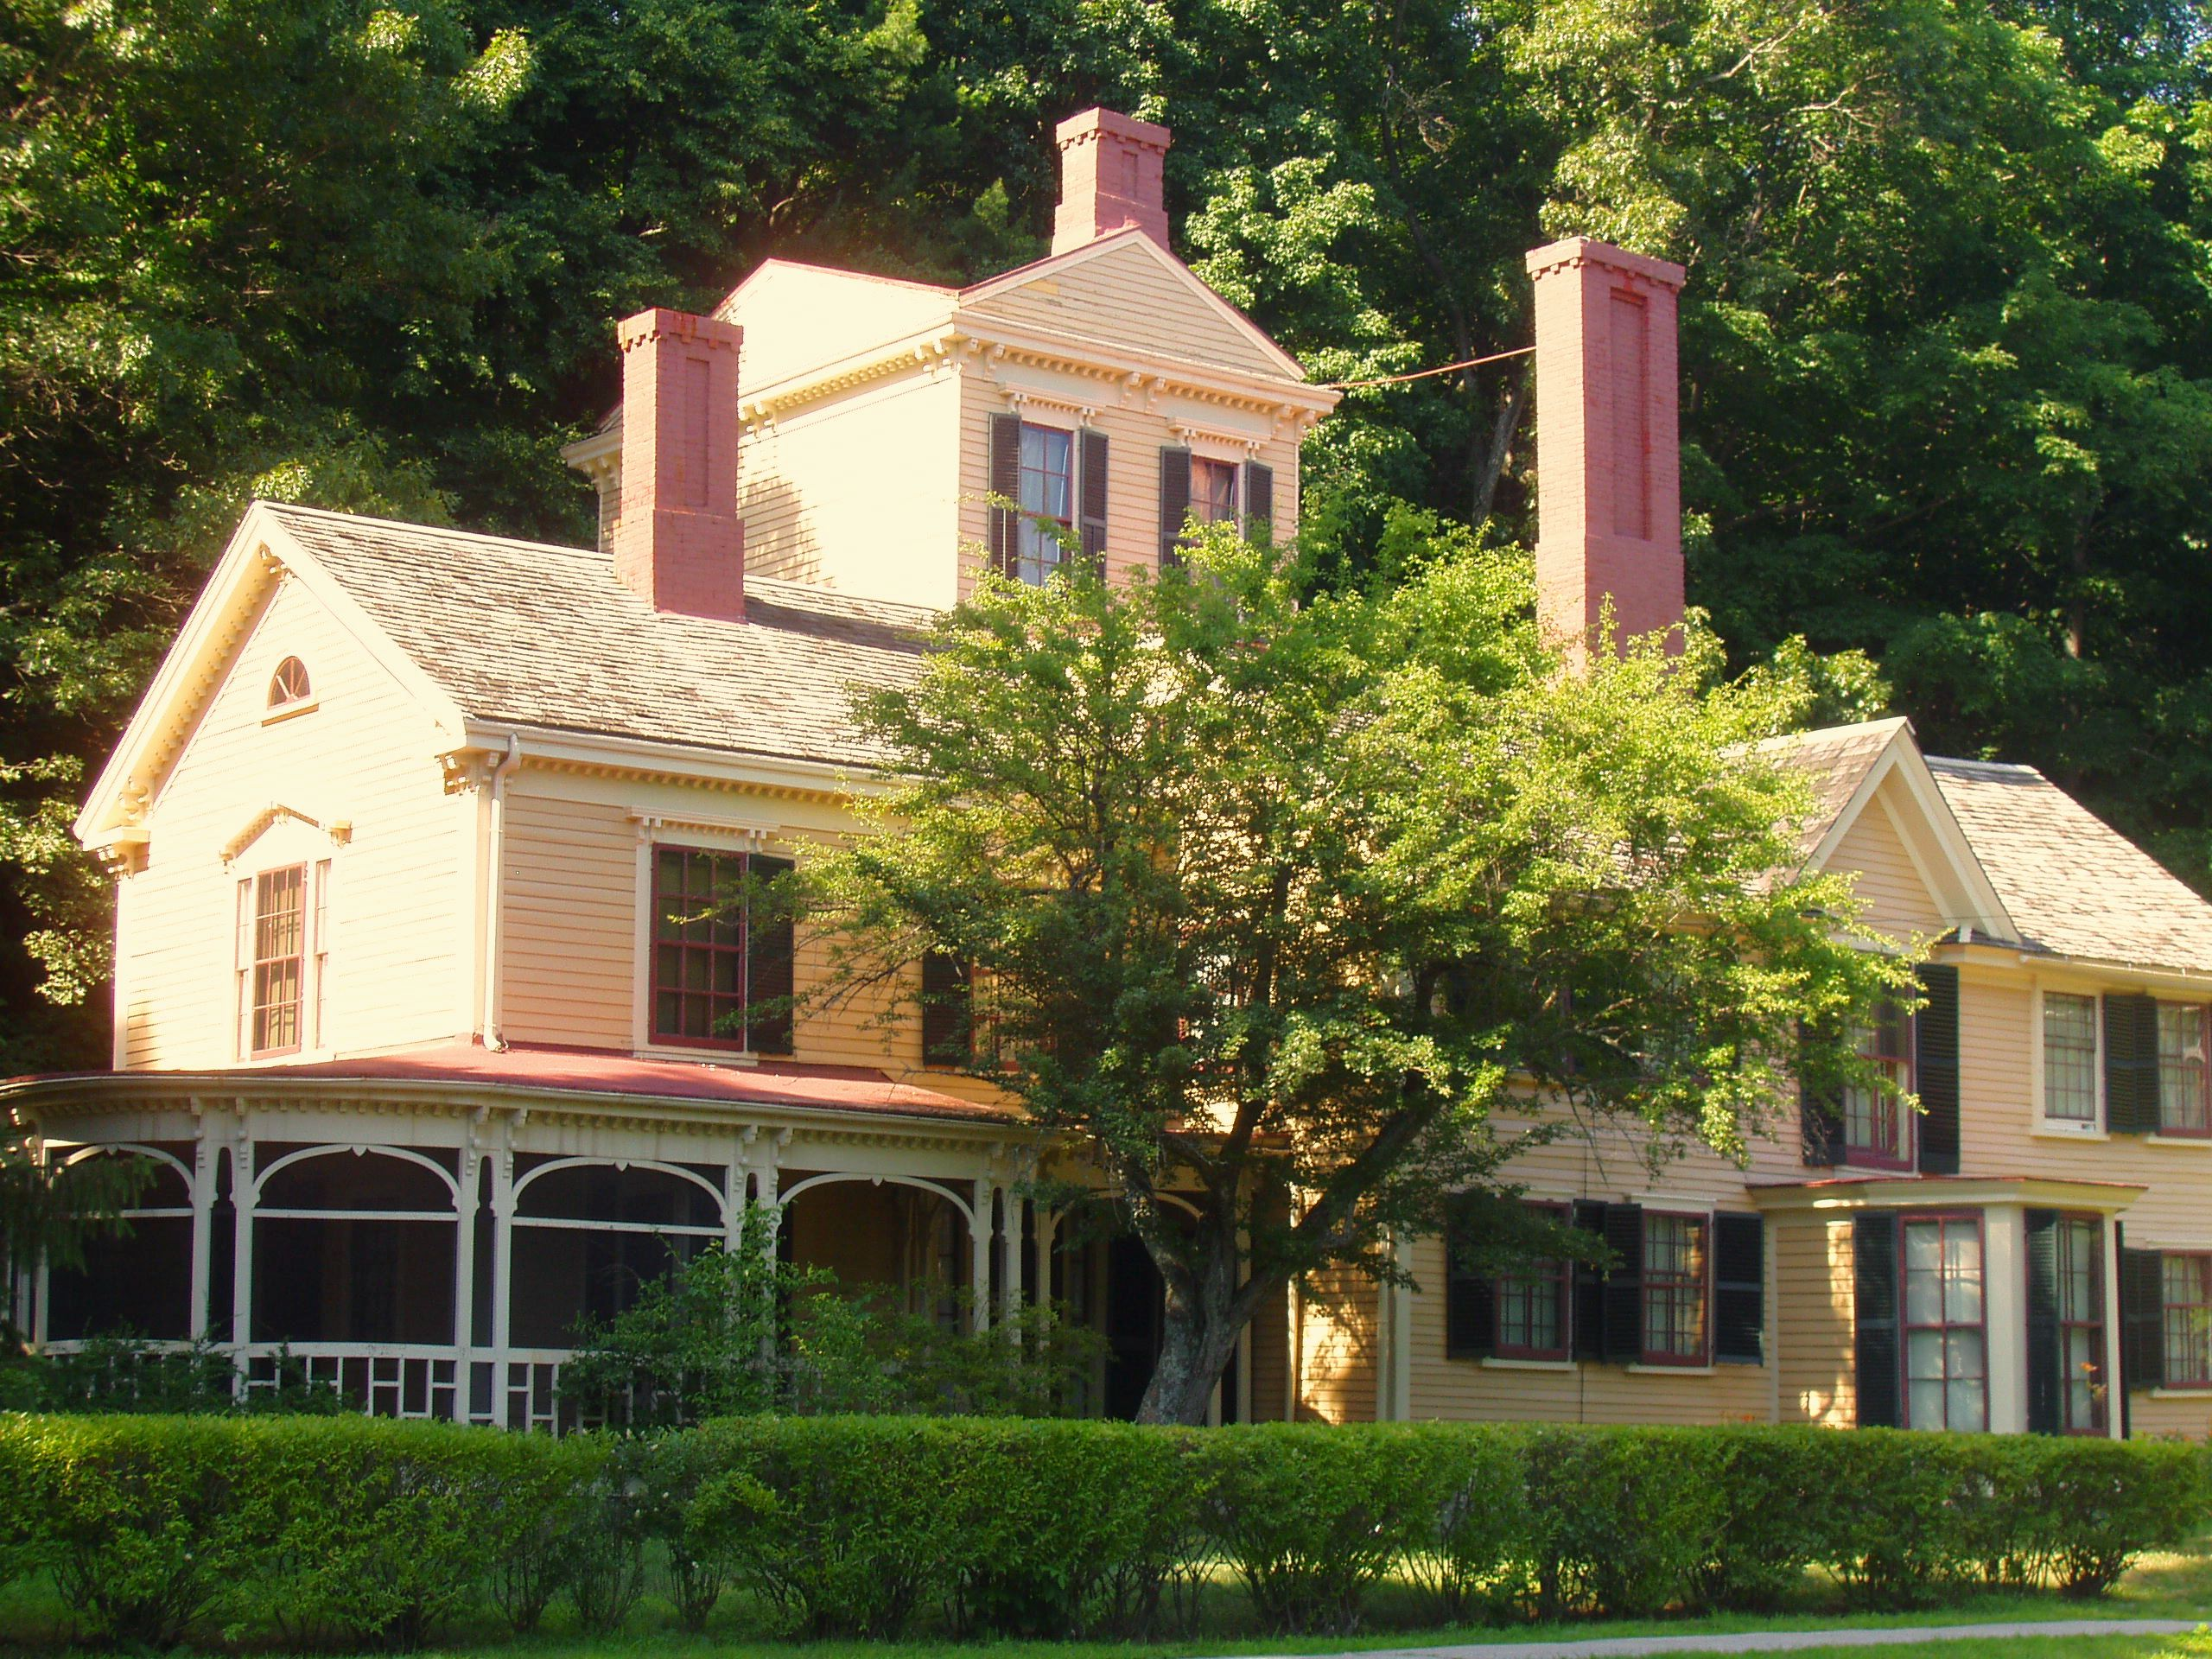
\includegraphics[width=.7\textwidth]{images/The_Wayside_Concord_Massachusetts}
% http://en.wikipedia.org/wiki/File:The_Wayside_Concord_Massachusetts.jpg
  \end{center}
\hfill (Daderot, Wikimedia Commons)

\end{frame}
%%%%%%%%%%%%%%%%%%%%%%%%%%%%%%%%%%%%%%%%%%%%%%%%%%%%%%%%%%%%%%%%%%%%%%%%%%%%%%%%

%%%%%%%%%%%%%%%%%%%%%%%%%%%%%%%%%%%%%%%%%%%%%%%%%%%%%%%%%%%%%%%%%%%%%%%%%%%%%%%%
\begin{frame}
  \frametitle{It's Not Just Software}


Nathaniel Hawthorne wrote:

\begin{quote}
I have been equally unsuccessful in my architectural projects; and have transformed a simple and small old farm-house into the absurdest anomaly you ever saw; but I really was not so much to blame here as the \sout{programmer} village-carpenter, who took the matter into his own hands, and produced an unimaginable sort of thing instead of what I asked for. (January 1864)
\end{quote}


\begin{tabular}{lrr}
Original budget:& \$500 &(\$7540 inflation-adjusted)\\
Actual cost: &\$2000 &(\$30160 inflation-adjusted)
\end{tabular}



\end{frame}
%%%%%%%%%%%%%%%%%%%%%%%%%%%%%%%%%%%%%%%%%%%%%%%%%%%%%%%%%%%%%%%%%%%%%%%%%%%%%%%%

%% Using locks also involves a trade-off between coarse-grained locking,
%% which can significantly reduce opportunities for parallelism, and
%% fine-grained locking, which requires more careful design, increases
%% locking overhead and is more prone to bugs.


%%%%%%%%%%%%%%%%%%%%%%%%%%%%%%%%%%%%%%%%%%%%%%%%%%%%%%%%%%%%%%%%%%%%%%%%%%%%%%%%
\begin{frame}
  \frametitle{Locking}

  
  Locks prevent data races.

  \begin{itemize}
    \item Locks' extents constitute their {\bf granularity}---do you lock large sections of your program with a big lock, or do you divide the locks and protect smaller sections?
  \end{itemize}

  Concerns when using locks:

  \begin{itemize}
    \item overhead;
    \item contention; and
    \item deadlocks.
  \end{itemize}
  
\end{frame}
%%%%%%%%%%%%%%%%%%%%%%%%%%%%%%%%%%%%%%%%%%%%%%%%%%%%%%%%%%%%%%%%%%%%%%%%%%%%%%%%

%%%%%%%%%%%%%%%%%%%%%%%%%%%%%%%%%%%%%%%%%%%%%%%%%%%%%%%%%%%%%%%%%%%%%%%%%%%%%%%%
\begin{frame}
  \frametitle{Locking: Overhead}

  

  Using a lock isn't free. You pay:
  \begin{itemize}
    \item allocated memory for the locks;
    \item initialization and destruction time; and
    \item acquisition and release time.
  \end{itemize}

  These costs scale with the number of locks that you have.
  
\end{frame}
%%%%%%%%%%%%%%%%%%%%%%%%%%%%%%%%%%%%%%%%%%%%%%%%%%%%%%%%%%%%%%%%%%%%%%%%%%%%%%%%

%%%%%%%%%%%%%%%%%%%%%%%%%%%%%%%%%%%%%%%%%%%%%%%%%%%%%%%%%%%%%%%%%%%%%%%%%%%%%%%%
\begin{frame}
  \frametitle{Locking: Contention}

  
    Most locking time is wasted waiting for the lock to become available.

    How can we fix this?
      \begin{itemize}
        \item Make the locking regions smaller (more granular);
        \item Make more locks for independent sections.
      \end{itemize}
  
\end{frame}
%%%%%%%%%%%%%%%%%%%%%%%%%%%%%%%%%%%%%%%%%%%%%%%%%%%%%%%%%%%%%%%%%%%%%%%%%%%%%%%%

%%%%%%%%%%%%%%%%%%%%%%%%%%%%%%%%%%%%%%%%%%%%%%%%%%%%%%%%%%%%%%%%%%%%%%%%%%%%%%%%
\begin{frame}
  \frametitle{Locking: Deadlocks}

  
  The more locks you have, the more you have to worry about deadlocks.\\[1em]

  Key condition: \\ 
\qquad waiting for a lock held by process $X$ \\while holding
a lock held by process $X'$. ($X = X'$ allowed).
  

\end{frame}
%%%%%%%%%%%%%%%%%%%%%%%%%%%%%%%%%%%%%%%%%%%%%%%%%%%%%%%%%%%%%%%%%%%%%%%%%%%%%%%%



\begin{frame}
\frametitle{Formal Deadlock Definition}

The four conditions for deadlock are:

\begin{enumerate}
	\item \textbf{Mutual Exclusion}
	\item \textbf{Hold-and-Wait}
	\item \textbf{No Preemption}
	\item \textbf{Circular-Wait}
\end{enumerate}



\end{frame}

%%%%%%%%%%%%%%%%%%%%%%%%%%%%%%%%%%%%%%%%%%%%%%%%%%%%%%%%%%%%%%%%%%%%%%%%%%%%%%%%
\begin{frame}[containsverbatim]
  \frametitle{Does this look familiar?}

  
     Consider two processors trying to get two {\it locks}:
     
     \vfill
  \begin{columns}
    \column{0.4\textwidth}
      {\bf Thread 1}

      \verb+Get Lock 1+

      \verb+Get Lock 2+

      \verb+Release Lock 2+

      \verb+Release Lock 1+
    \column{0.4\textwidth}
      {\bf Thread 2}

      \verb+Get Lock 2+

      \verb+Get Lock 1+

      \verb+Release Lock 1+

      \verb+Release Lock 2+
    \end{columns}~\\[1em]
     Processor 1 gets Lock 1, then Processor 2 gets Lock 2. Oops!
          They both wait for each other \structure{(deadlock)}.
  
\end{frame}
%%%%%%%%%%%%%%%%%%%%%%%%%%%%%%%%%%%%%%%%%%%%%%%%%%%%%%%%%%%%%%%%%%%%%%%%%%%%%%%%

%%%%%%%%%%%%%%%%%%%%%%%%%%%%%%%%%%%%%%%%%%%%%%%%%%%%%%%%%%%%%%%%%%%%%%%%%%%%%%%%
\begin{frame}
  \frametitle{Key to Preventing Deadlock}

  

  Always be careful if \\
your code {\bf acquires a lock while holding one}.\\[1em]

  Here's how to prevent a deadlock:
  
  \begin{itemize}
    \item Ensure consistent ordering in acquiring locks; or
    \item Use {\tt trylock}.
  \end{itemize}
  
\end{frame}
%%%%%%%%%%%%%%%%%%%%%%%%%%%%%%%%%%%%%%%%%%%%%%%%%%%%%%%%%%%%%%%%%%%%%%%%%%%%%%%%

%%%%%%%%%%%%%%%%%%%%%%%%%%%%%%%%%%%%%%%%%%%%%%%%%%%%%%%%%%%%%%%%%%%%%%%%%%%%%%%%
\begin{frame}[fragile]
  \frametitle{Preventing Deadlocks---Ensuring Consistent Ordering}

  
  \begin{lstlisting}
void f1() {
    lock(&l1);
    lock(&l2);
    // protected code
    unlock(&l2);
    unlock(&ll);    
}

void f2() {
    lock(&l1);
    lock(&l2);
    // protected code
    unlock(&l2);
    unlock(&ll);    
}
  \end{lstlisting}

     This code will not deadlock: you can only get {\bf l2} if you have
      {\bf l1}.
  
\end{frame}
%%%%%%%%%%%%%%%%%%%%%%%%%%%%%%%%%%%%%%%%%%%%%%%%%%%%%%%%%%%%%%%%%%%%%%%%%%%%%%%%



\begin{frame}
\frametitle{Formal Lock Ordering}


If the set of all resources in the system is $R = \{R_{0}, R_{1}, R_{2}, ... R_{m}\}$:

Assign to each resource $R_{k}$ a unique integer value. Let us define this function as $f(R_{i})$, that maps a resource to an integer value. 

This integer value is used to compare two resources: if a process has been assigned resource $R_{i}$, that process may request $R_{j}$ only if $f(R_{j}) > f(R_{i})$. 

If the process needs more than one of $R_{i}$ then the request for all of these must be made at once (in a single request). 

To get $R_{i}$ when already in possession of a resource $R_{j}$ where $f(R_{j}) > f(R_{i})$, the process must release any resources $R_{k}$ where $f(R_{k}) \geq f(R_{i})$. 

If these two protocols are followed, then a circular-wait condition cannot hold.



\end{frame}

%%%%%%%%%%%%%%%%%%%%%%%%%%%%%%%%%%%%%%%%%%%%%%%%%%%%%%%%%%%%%%%%%%%%%%%%%%%%%%%%
\begin{frame}[fragile]
  \frametitle{Preventing Deadlocks---Using {\tt trylock}}

  
  Recall: Pthreads' {\tt trylock} returns 0 if it gets the lock.

  \begin{lstlisting}
void f1() {
    lock(&l1);
    while (trylock(&l2) != 0) {
        unlock(&l1);
        // wait
        lock(&l1);
    }
    // protected code
    unlock(&l2);
    unlock(&ll);    
}
  \end{lstlisting}

    This code also won't deadlock: it will give up {\bf l1} if it can't get
    {\bf l2}.\\[1em]

    (BTW: trylocks also enable measuring lock contention.)

  
\end{frame}
%%%%%%%%%%%%%%%%%%%%%%%%%%%%%%%%%%%%%%%%%%%%%%%%%%%%%%%%%%%%%%%%%%%%%%%%%%%%%%%%

%%%%%%%%%%%%%%%%%%%%%%%%%%%%%%%%%%%%%%%%%%%%%%%%%%%%%%%%%%%%%%%%%%%%%%%%%%%%%%%%
\begin{frame}
  \frametitle{Coarse-Grained Locking (1)}

  \begin{center}
    
\includegraphics[scale=0.5]{images/lock-all-the-things}

    (with one lock)
  \end{center}
\end{frame}
%%%%%%%%%%%%%%%%%%%%%%%%%%%%%%%%%%%%%%%%%%%%%%%%%%%%%%%%%%%%%%%%%%%%%%%%%%%%%%%%

%%%%%%%%%%%%%%%%%%%%%%%%%%%%%%%%%%%%%%%%%%%%%%%%%%%%%%%%%%%%%%%%%%%%%%%%%%%%%%%%
\begin{frame}
  \frametitle{Coarse-Grained Locking (2)}

  
  {\bf Advantages:}
  
  \begin{itemize}
    \item Easier to implement;
    \item No chance of deadlocking;
    \item Lowest memory usage / setup time.
  \end{itemize}
  \vfill
  {\bf Disadvantages:}
  \begin{itemize}
    \item Your parallel program can quickly become sequential.
  \end{itemize}
  
\end{frame}
%%%%%%%%%%%%%%%%%%%%%%%%%%%%%%%%%%%%%%%%%%%%%%%%%%%%%%%%%%%%%%%%%%%%%%%%%%%%%%%%

%%%%%%%%%%%%%%%%%%%%%%%%%%%%%%%%%%%%%%%%%%%%%%%%%%%%%%%%%%%%%%%%%%%%%%%%%%%%%%%%
\begin{frame}
  \frametitle{Coarse-Grained Locking Example---Python GIL}

  
  This is the main reason (most) scripting languages have poor parallel
  performance; Python's just an example.

  \begin{itemize}
    \item Python puts a lock around the whole interpreter\\ \quad (global interpreter lock).

    \item Only performance benefit you'll see from threading is if a thread is
      waiting for IO.

    \item Any non-I/O-bound threaded program will be {\bf slower} than the sequential
      version (plus, it'll slow down your system).
  \end{itemize}
  
\end{frame}
%%%%%%%%%%%%%%%%%%%%%%%%%%%%%%%%%%%%%%%%%%%%%%%%%%%%%%%%%%%%%%%%%%%%%%%%%%%%%%%%

%%%%%%%%%%%%%%%%%%%%%%%%%%%%%%%%%%%%%%%%%%%%%%%%%%%%%%%%%%%%%%%%%%%%%%%%%%%%%%%%
\begin{frame}
  \frametitle{Fine-Grained Locking (1)}

  \begin{center}
    
\includegraphics[scale=0.5]{images/lock-all-the-things}

    (with all different locks)
  \end{center}
\end{frame}
%%%%%%%%%%%%%%%%%%%%%%%%%%%%%%%%%%%%%%%%%%%%%%%%%%%%%%%%%%%%%%%%%%%%%%%%%%%%%%%%

%%%%%%%%%%%%%%%%%%%%%%%%%%%%%%%%%%%%%%%%%%%%%%%%%%%%%%%%%%%%%%%%%%%%%%%%%%%%%%%%
\begin{frame}
  \frametitle{Fine-Grained Locking (2)}

  
  {\bf Advantages:}
  
  \begin{itemize}
    \item Maximizes parallelization in your program.
  \end{itemize}
  \vfill
  {\bf Disadvantages}
  \begin{itemize}
    \item May be mostly wasted memory / setup time.
    \item Prone to deadlocks.
    \item Generally more error-prone (be sure you grab the right lock!)
  \end{itemize}
  
\end{frame}
%%%%%%%%%%%%%%%%%%%%%%%%%%%%%%%%%%%%%%%%%%%%%%%%%%%%%%%%%%%%%%%%%%%%%%%%%%%%%%%%

%%%%%%%%%%%%%%%%%%%%%%%%%%%%%%%%%%%%%%%%%%%%%%%%%%%%%%%%%%%%%%%%%%%%%%%%%%%%%%%%
\begin{frame}
  \frametitle{Fine-Grained Locking Examples}

  
    The Linux kernel used to have {\bf one big lock}\\ that essentially made
      the kernel sequential. 
    \begin{itemize}
      \item (worked fine for single-processor systems!)
    \end{itemize}
    Now uses finer-grained locks for performance.\\[2em]

    Databases may lock fields / records / tables.\\
    \qquad  (fine-grained $\rightarrow$ coarse-grained).\\[1em]

    Can lock individual objects.
  

\end{frame}
%%%%%%%%%%%%%%%%%%%%%%%%%%%%%%%%%%%%%%%%%%%%%%%%%%%%%%%%%%%%%%%%%%%%%%%%%%%%%%%%



\section{}
%%%%%%%%%%%%%%%%%%%%%%%%%%%%%%%%%%%%%%%%%%%%%%%%%%%%%%%%%%%%%%%%%%%%%%%%%%%%%%%%
\begin{frame}
  \frametitle{Summary}

  
 C++11 memory model.\\
 
 Good increment practice. \\

 Lock granularity.

  
\end{frame}
%%%%%%%%%%%%%%%%%%%%%%%%%%%%%%%%%%%%%%%%%%%%%%%%%%%%%%%%%%%%%%%%%%%%%%%%%%%%%%%%

\end{document}

